\section{Deep Learning}
This section introduces deep neural networks, recurrent neural networks, and
reinforcement learning. They are the machine learning tools that we use in
\cref{chap:dopey} and \cref{chap:doccam}.
\begin{figure*}[t]
  \centering
  \begin{subfigure}[t]{0.3\textwidth}
    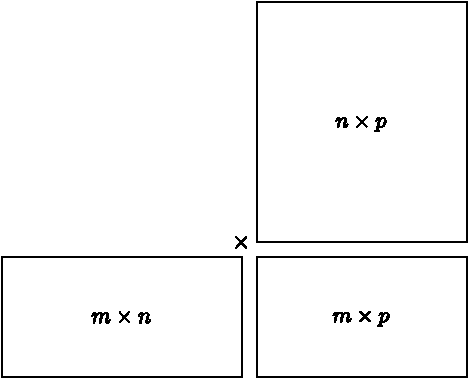
\includegraphics[width=0.99\textwidth]{figures/matmul.pdf}
    \caption{Matrix multiplication.}
    \label{fig:matmul}
	\end{subfigure}
	\begin{subfigure}[t]{0.3\textwidth}
    \adjincludegraphics[width=0.99\textwidth, trim={0 {.08\height} 0 0},clip]{figures/perceptron.pdf}
    \caption{Perceptron}
    \label{fig:perceptron}
	\end{subfigure}
	\begin{subfigure}[b]{0.6\textwidth}
    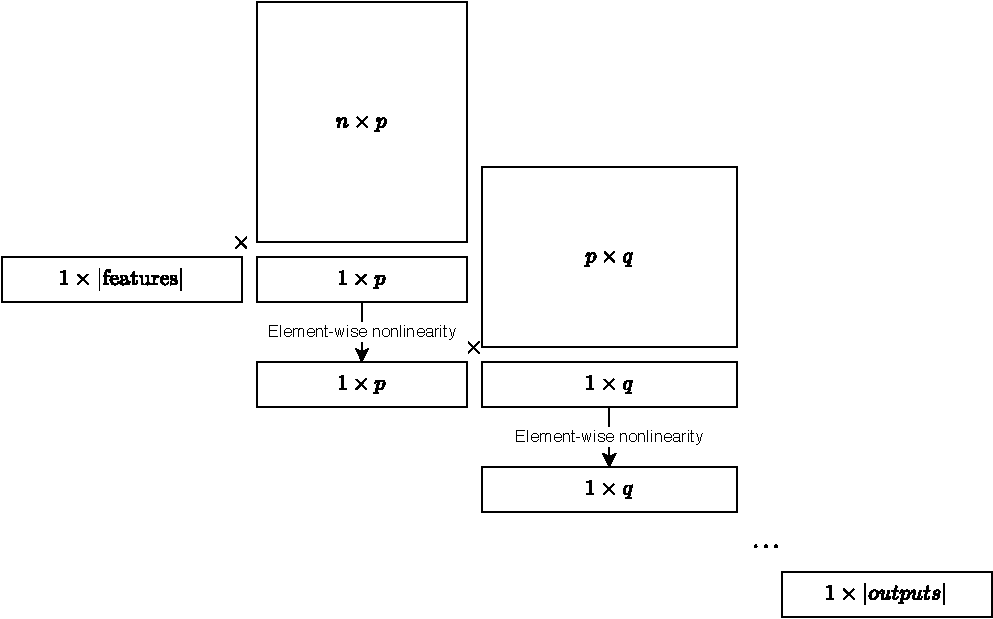
\includegraphics[width=0.99\textwidth]{figures/deep_matmul.pdf}
    \caption{Multi-layer Perceptron}
    \label{fig:deep_matmul}
	\end{subfigure}
	\begin{subfigure}[b]{0.6\textwidth}
    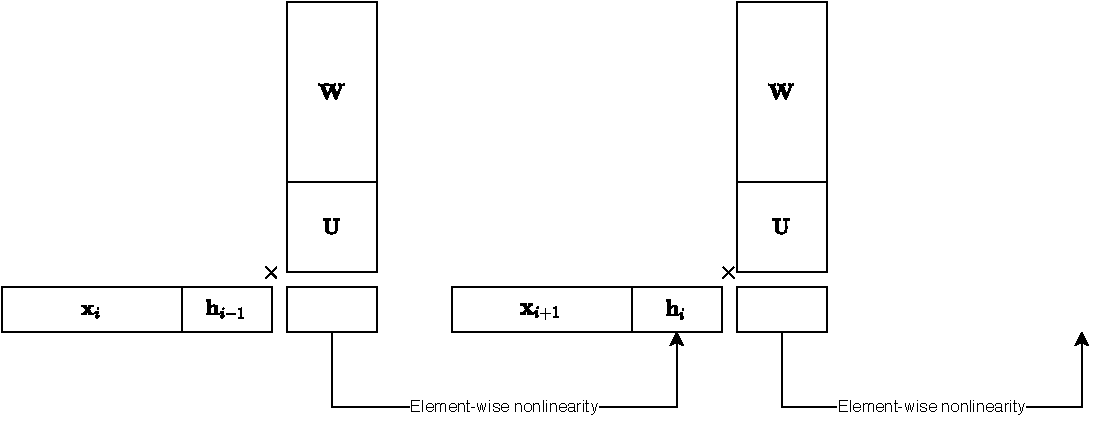
\includegraphics[width=0.99\textwidth]{figures/RNN.pdf}
    \caption{Recurrent neural network}
    \label{fig:rnn}
	\end{subfigure}  \caption{Visualization of matrix multiplication, perceptron,
    multi-layer perceptron, and recurrent neural network.}
\end{figure*}
\subsection{Perceptron. Multi-layer Perceptron. The fixed-size computing paradigm.}
There are already too many technical texts about the mathematical behind
Perceptron and Multi-layer Perceptron. In this section, we take a pictorial
look at it, starting from matrix multiplication. Multiplying two matrices of
size $m \times n$ and $n \times p$ could be visualized as in \cref{fig:matmul},
which resulted in a new matrix of size $m \times p$.

\paragraph{Perceptron} is defined as a function that maps its input $\vect{x}$
(a real-valued vector) to an output value $y$ (a single binary value). While
there are many ways to define the mapping, in practice the perceptron function is
\begin{align*}
  y =  \twopartdef { 1 } {\vect{x} \times \vect{W} + \text{bias} > 0} 
                   { 0 } {\text{otherwise}}
\end{align*}
\cref{fig:perceptron} visualizes the perceptron function. In case of having to
classify $k$ classes ($k>2$), a one-vs-all scheme is used: learn $k$ separated
perceptron, each perceptron $p_i$ predicts whether $\vect(x)$ is of the class
$i^{th}$.

In the early 60s, it is believed that Single-layer perceptron was all we needed to learn
(approximate) any function. In 1969, Minsky and Papert \cite{perceptrons} proved
that a single perceptron cannot learn the simple XOR function, since XOR is not
\emph{linear separable}. There work effectively froze AI research for about ten years.

The solution for the XOR function, as it turned out, was very simple:
Multi-layer Perceptrons.

\paragraph{Multi-layer Perceptron.} To understand Multi-layer Perceptron, let's
take a step back and look at what a Single-layer Perceptron does: it computes a linear
transformation of the input ($\vect{x} \times \vect{W} + \text{bias}$), then
applies a non-linear filter (activation function) over the results (a branching function). The key
insight is that the result is also a matrix, hence can be feed into another
perceptron, which in total, make a non-linear function! In fact, it is proven \cite{universal}
that under certain assumptions, 2 layer perceptrons is enough to approximate arbitrary
functions!

\cref{fig:deep_matmul} visualizes a multi-layer perceptron. Looking at the
figure, it is also clear why it is also called \emph{Deep Learning}. One way to
think about Deep Learning: given a dataset $\cD$ of pairs $(\vect{x}_i, y_i)$, what
is a good architecture (the arrangement of intermediate matrices), and what are
the values for entries in the matrices?

\paragraph{The fixed-size computing paradigm.} Multi-layer perceptrons are
great, and could be used to approximate many functions. But it also forces
things to be in the same shape: once the architecture is fixed, all the matrices
in between are also fixed in shape, so all inputs have to have the same shape,
and all outputs also have to have the same shape as well. For many cases, this
is not a big problem: image could be resized into a fixed size, missing
values in an input vector could always be set to a dummy values, for examples.
But in some cases, the whole paradigm just doesn't work, and requires a
different paradigm altogether. 


\subsection{Recurrent-neural network. Tree LSTM.}
In many tasks, we need to process inputs of arbitrary length, to predict outputs also of arbitrary length (often called \emph{sequence-to-sequence} problems). There are multiple ways to make sequential inputs to work in the fixed-size paradigm, such as \emph{padding} (add dummy values to the inputs to make sure they are all of the same length), \emph{same length batching} (sort inputs by size and process inputs of the same size together), among others. However, those approaches doesn't help with handling sequential outputs. A better approach is \emph{recurrent neural networks} (RNNs). An RNN defines a function
\begin{align}
\vect{h}^t = f(\vect{h}^{t-1}, \vect{x}^{t})
\end{align}
in which $f$ is our linear transformation, followed by a non-linear filter. A
typical RNN can be
\begin{align}
  f(\vect{h}^{t-1}, \vect{x}^t) = tanh(\vect{x}_t \times \vect{W} + \vect{h}_{t-1} \times \vect{U} )
\end{align}
This simple RNN is visualized in \cref{fig:rnn}. Note that $\vect{W}$ and
$\vect{U}$ are shared. This also means that the longer the chain, the easier it
is for the first input to vanish/explode in the computation of the current
input, since $\vect{h}_t$ has the term $\vect{x}_0\times\vect{W}^t$ in it.
In practice, vanilla RNNs rarely can learn for chains longer than 10 time steps.

To address this issue, a forget/gating mechanism is added to RNN, most notably
in architecture like LSTM \cite{lstm} and GRU \cite{gru}. Equations to compute
the output (update) at the time step $t$  for LSTM
with a forget gate are:
\begin{align}
  \vf_t &= \sigma(\vect{x}_t \times \vect{W}_f + \vect{h}_{t-1} \times \vect{U}_f + \text{bias}_f)\\
  \vi_t &= \sigma(\vect{x}_t \times \vect{W}_i + \vect{h}_{t-1} \times \vect{U}_i + \text{bias}_i)\\
  \vo_t &= \sigma(\vect{x}_t \times \vect{W}_o + \vect{h}_{t-1} \times \vect{U}_o + \text{bias}_o)\\
  \va_t &= \tanh{(\vect{x}_t \times \vect{W}_a + \vect{h}_{t-1} \times \vect{U}_a + \text{bias}_a)}\\
  \vc_t &= \vf_t \circ \vc_{t-1} + \vi_t \circ \va_t \\
  \vh_t &= \vo_t \circ \tanh{(\vc_t)}
\end{align}
where $\sigma$ is the sigmoid activation function, and $\circ$ is the
element-wise product.

\paragraph{TreeLSTM}
While LSTM works well on a sequence of inputs, it doesn't explicitly work with a
tree of inputs, such as an Abstract Syntax Tree (AST). One can force LSTM to work with a tree like of inputs by
flattening the tree into a sequence of tokens, but this normally requires adding
more separator tokens (like brackets) into the sequence, making if inefficient.
A better way is to directly enforce the tree structure into the update
equations, which was introduced in \cite{TreeLSTM}. Given a tree, let $C^j$
denote the set of children of node $j$. The Child-Sum TreeLSTM update equations
are:
\begin{align}
  \vs_j &= \sum_{k\in C^j}{\vh_k} \label{eq:summation}\\
  \vf_{jk} &= \sigma(\vect{x}_j \times \vect{W}_f + \vect{h}_{k} \times \vect{U}_f + \text{bias}_f)\\
  \vi_j &= \sigma(\vect{x}_j \times \vect{W}_i + \vect{s}_{j} \times \vect{U}_i + \text{bias}_i)\label{eq:tree-lstm-update-i}\\
  \vo_j &= \sigma(\vect{x}_j \times \vect{W}_o + \vect{s}_{j} \times \vect{U}_o + \text{bias}_o)\label{eq:tree-lstm-update-o}\\
  \va_j &= \tanh{(\vect{x}_j \times \vect{W}_a + \vect{s}_{j} \times \vect{U}_a + \text{bias}_a)}\label{eq:tree-lstm-update-a}\\
  \vc_j &= \vi_j \circ \va_{j} + \sum_{k \in C^j}{\vf_{jk} \circ \vc_k} \\
  \vh_j &= \vo_j \circ \tanh{(\vc_j)}
\end{align}
Intuitively, TreeLSTM incorporates the \emph{summation} of outputs of children
(\cref{eq:summation}) into the computation of the parent node
(in \cref{eq:tree-lstm-update-i} to \cref{eq:tree-lstm-update-a}, TreeLSTM uses
$\vs$ instead of $\vh$ as in vanilla LSTM), which enforces the tree structure.
Note that TreeLSTM is a generalized version of vanilla LSTM: if each node has exactly one child, we get the same equations as in
vanilla LSTM.
%% Recurrent neural networks (RNNs) are widely used in natural language processingtasks, especially speech recognition and machine translation. The primary goal ofRNNs is to approximate the mapping from a sequence of inputsx(1),...,x(t)to eithera single outputyor a sequence of outputsy(1),...,y(t). An RNN defines a mappingh(t)=f(h(t−1),x(t);θ)(2.2)whereh(t)is the hidden state, from which the final outputy(t)can be computed byeither a non-linear transformation or an MLP.11
%% Popular RNN models.A simple RNN model can be. The key issue of such a simple form is that the long-termdependencies are hard to capture, which makes training extremely difficult. Toaddress this issue, a commonly used RNN model is the long short-term memorynetwork (LSTM) [89], which introduces amemory cell with various gatesto preservestate over a long sequence.LSTM maintains two states — the original hidden state and a newly introducedcontextstate (or memory cell). At a high level, LSTM defines a mapping functionas follows:h(t),c(t)=f(h(t−1),c(t−1),x(t);θ)(2.4)whereh(t)is the hidden state andc(t)is the context state. These two states areupdated by three gates — input gatei(t), forget gatef(t)and output gateo(t)asfollows:i(t)=σ(Wix(t)+Uih(t−1)+bi)f(t)=σ(Wfx(t)+Ufh(t−1)+bf)o(t)=σ(Wox(t)+Uoh(t−1)+bo)u(t)=tanh(Wux(t)+Uuh(t−1)+bu)c(t)=i(t)u(t)+f(t)c(t−1)h(t)=o(t)tanh(c(t))(2.5)whereθ=  [Wi,Ui,bi,Wf,Uf,bf,Wo,Uo,bo,Wu,Uu,bu],σis the sigmoid function,andis the element-wise product.Two common variants of LSTM are gated recurrent units (GRUs) [41] and tree-structured LSTM (Tree-LSTM) [177]. The former simplifies gates of LSTM for effi-ciency while the latter extends the modeling ability to tree structures.12

\subsection{Reinforcement learning}
% In many tasks, the learning goal is beyond predicting some predefined label for a given input. Instead, the learning goal is to reach some beneficial state after a se- quence of actions following a set of rules from some initial state. Thus, what is really learned is a policy, which predicts an action given a state and the action is ideally optimal towards the ultimate beneficial state. Reinforcement learning is a system- atic methodology of solving this exact problem and has achieved remarkable suc- cesses in many challenging problems, particularly games. Prominent examples are strategical games like Chess [93] and Go [166], and video games like Atari [124], StarCraft [179], and Dota [132].
In many tasks, a dataset of input-output pairs $(\vec{x}, y)$ is too expensive,
or even impossible to obtain: imagine having to label all the best moves for
half of the number of all possible chess boards! More importantly, in many
cases, we do not really need one single correct output, but many possible
outputs are equally good, as long as their cumulative effects are the same: as
long as we reach the destination in time, it doesn't really matter whether our
speed at time $t$ is 40 or 50 km/h. To solve those two problems, we need to have
a learning paradigm that optimizes for a global \emph{goal}, while collecting
the data all by itself. \emph{Reinforcement learning} is such a paradigm, and
has achieved remarkable successes in many difficult tasks, such as Robotics
\cite{convai} or playing board games \cite{td-gammon, alphago}.

\paragraph{Markov Decision Process.} A standard formulation of RL is using
Markov decision process (MDP):
\begin{itemize}
  \item A set of states $S$;
  \item a set of actions $A$;
  \item $P_a(s, s') = Pr(s_{t+1} = s' \mid s_t = s, a_t = a)$ is the probability
    a state $s$ transits to another state $s'$, by taking the action $a$;
  \item $R_a(s, s')$ is the reward \emph{after} the transition from $s$ to $s'$ by
    taking the action $a$.  
\end{itemize}
At each time step $t$, the system interacts with its environment and receives
the current state $s_t$ and the immediate reward $r_t$. The goal of RL is to
learn a policy $\pi: A \times S \mapsto [0, 1], \pi(a, s) = Pr(a_t=a|s_t=s)$
that defines the probability of taking an action $a$ when in state $s$. Note
that in this thesis, we only care about finite action spaces (discrete actions).
There is also continuous action spaces, i.e predicting the
optimal speed at each time step. We want $\pi$ to maximize the expected
cumulative reward. In our setting, where $P$ is deterministic (taking one action
results in only one possible new state), the cumulative
reward is defined as:
\begin{align}
  E = \sum_{t=0}^{T-1}{R_{a_t}(s_t, s_{t+1})}
\end{align}
where $T$ could be $\infty$ if necessary.

The dilemma of RL lies in the fact that we often do not have access to the true
reward function $R$ (if we do, we can simply sample many tuple $(s, a,
R_a(s))$ and learn it in a supervised manner), only the final reward at the
end of the execution of the policy, but in practice RL cannot be trained without
intermediate feed backs. For example, imagine if we can only train a Chess RL system if the
only reward is a binary signal at the end! Hence, a big part of RL research is
about crafting adequate \emph{proxy rewards}, that tells the agent how well
it currently performing. One can directly craft the proxies using domain
knowledge, such as assigning scores for board configurations in Chess, or use
best-so-far random policy as the target (e.g Policy Gradient \cite{reinforce}), or learn the reward
function for a state-action pair instead of the reward for just the state
(e.g Deep-Q learning \cite{deepq}).